\apendice{Plan de Proyecto Software}

\section{Introducción}
A la hora de abordar un proyecto relativamente complejo como este, el primer paso debe ser definir la metodología de trabajo que se va a emplear durante su desarrollo, es decir, qué criterio se va a seguir para dividir el proyecto en tareas más sencillas, y cómo se organizarán estas en términos de alcance y temporalidad.
\section{Planificación temporal}
\subsection{Herramientas y conceptos}
En este proyecto se ha utilizado GitHub \cite{wiki:Github} como herramienta principal para la gestión de versiones y como gestor de la planificación temporal.

La planificación temporal En GitHub se construye mediante piezas llamadas tareas o \textit{Issues} (ver figura \ref{fig:TareasGithub}).
\begin{figure}[h]
	\centering
	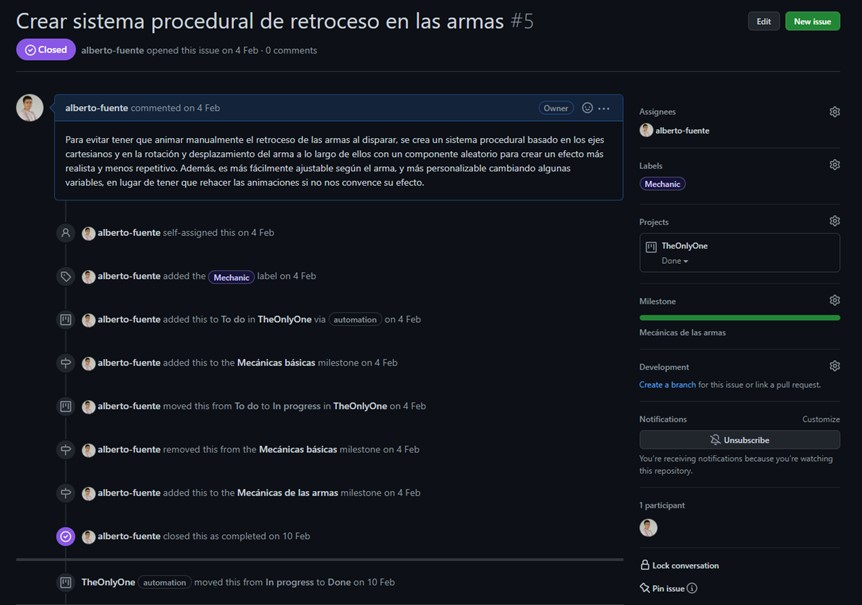
\includegraphics[scale=0.45]{img/GithubScreenshot.jpg}
	\caption{Captura de una tarea en Github}
	\label{fig:TareasGithub}
    \end{figure}
Las tareas representan una acción o pequeño conjunto de acciones relacionadas que han de llevarse a cabo en el proyecto para solventar un problema, crear una mecánica o cumplir un requerimiento. Es decir, son subdivisiones que se hacen del proyecto para poder gestionarlo de forma más eficiente.

Cada tarea se compone de los siguientes elementos:
\begin{itemize}
    \item \textbf{Nombre}: Define en pocas palabras el objetivo de la tarea. 
    \item \textbf{Descripción}: Explica con más detalle en qué consiste la tarea y por qué es necesario teneral en cuenta.
    \item \textbf{Encargado}: Persona o personas que llevarán a cabo la tarea. En este caso, el alumno siempre será el encargado de todas las tareas.
    \item \textbf{Etiquetas}: Se pueden asignar una o varias etiquetas previamente definidas a cada tarea para tener un mejor control sobre ellas y saber de un vistazo a qué ámbito corresponden.\\
    Las etiquetas que se han definido para este proyecto son las siguientes:
    \begin{itemize}
        \item \textbf{Mechanic}. Tarea que forma parte de una mecánica del videojuego. Generalmente se asocia esta etiqueta a aspectos de programación.
        \item \textbf{Animation}. Tareas de animación de algún modelo o interfaz del videojuego.
        \item \textbf{Audio}. Tareas relacionadas con aspectos de sonido o música.
        \item \textbf{Bug}. Algún problema inesperado que requiera solución.
        \item \textbf{Change}. Cambio en algún aspecto o componente del videojuego.
        \item \textbf{Documentation}. Tareas relacionadas con la documentación del proyecto.
        \item \textbf{Enhancement}. Mejoras o nuevas características en algún componente del videojuego.
        \item \textbf{Modelling}. Trabajos de modelado de algún asset del videojuego.
        \item \textbf{UI}. Elementos visuales de la interfaz del usuario como los botones, el HUD o los menús.
        \item \textbf{VFX}. Efectos visuales como partículas o explosiones.
    \end{itemize}
    \item \textbf{Sprint/Milestone/Hito}: Es una agrupación de tareas con una fecha de finalización marcada. En principio, todas las tareas que conforman un sprint deben estar completadas al llegar a dicha marca temporal.\\
    Los sprints suelen ser utilizados en la metodología ágil SCRUM.
\end{itemize}
Los videojuegos son un tipo de proyecto en el que no todas las funcionalidades, mecánicas y contenido del juego están predefinidas antes de comenzar su desarrollo, sino que varias de estas características y apartados irán evolucionando a medida que se vaya desarrollando el juego (quizás porque surjan ideas nuevas, porque se modifiquen otras o porque se tengan que desechar aquellas que parecían buenas en un principio).

La magnitud del proyecto, sumado al hecho de que su desarrollo lo lleva a cabo una única persona, requiere ciclos de revisión rápidos y adaptables que hagan que la comprobación de tareas sea dinámica y flexible y permita una fácil gestión de estas.

Idealmente se debería permitir alargar o acortar la duración de estas si el proyecto así lo requiriese por cualquier motivo, ya que no es raro que los plazos se retrasen, por ejemplo, por culpa de un bug que no permita avanzar en una determinada parte del proyecto.\\ Esto es necesario para reducir al máximo el impacto que el retraso de una tarea pueda provocar al resto del proyecto.

Teniendo en cuenta todos estos factores, se decidió que la planificación temporal de este proyecto se haría a través de la metodología Kanban.

\textbf{\textit{Kanban}} \cite{wiki:Kanban} forma parte de las metodologías ágiles y se basa en el desarrollo y entrega continuos de un pequeño número de tareas de forma fluida y simultánea. Es muy útil en proyectos donde los cambios pueden suceder con facilidad, como es el caso.\\
Además, la metodología Kanban es muy visual, ya que gira en torno a un elemento llamado \textbf{tablero Kanban} (ver figura \ref{fig:TableroKanban}), un conjunto de columnas que conforman espacios para situar las diferentes tareas en función de su grado de completitud, creando un flujo de trabajo en el que se visualiza rápidamente el estado del proyecto.
\begin{figure}[h]
	\centering
	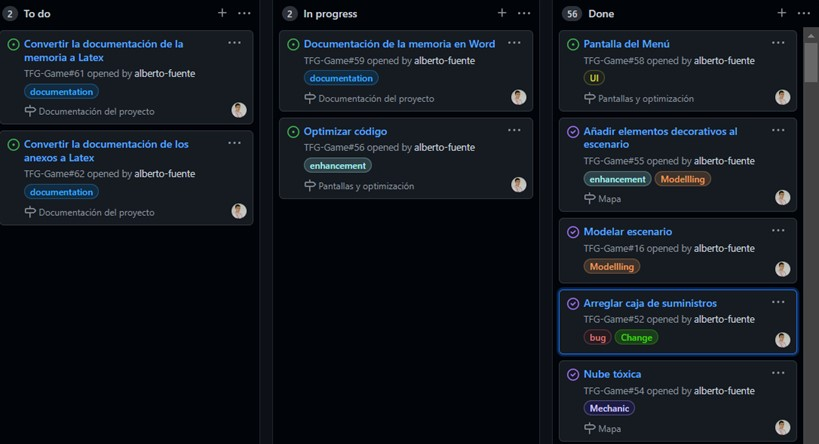
\includegraphics[scale=0.45]{img/KanbanBoard.jpg}
	\caption{Tablero Kanban de Github}
	\label{fig:TableroKanban}
    \end{figure}
Para este proyecto en particular, el tablero Kanban se ha implementado a través de la herramienta de GitHub situada en el apartado ``Projects''. Resulta muy conveniente, ya que se puede asociar el tablero al repositorio del proyecto, de tal manera que cada vez que se crea o modifica el estado de una tarea, aparecerá automáticamente una tarjeta del tablero Kanban.\\
Esto permite trabajar de manera mucho más cómoda y fluida a la hora de gestionar las tareas. 

En este caso, el tablero Kanban está formado por tres columnas y el flujo de estado de las diferentes tareas funciona de la siguiente manera:
\begin{itemize}
    \item \textbf{TO DO}: contiene las tareas que se tiene intención de realizar pero que no han comenzado aún. Cada vez que se crea una nueva tarjeta, se incluirá en esta columna.\\
    Al comienzo del proyecto se incluyen todas las tareas que previsiblemente precisará el proyecto. Sin embargo, algunas pueden ir surgiendo durante su transcurso a medida que se vaya necesitando definir nuevas tareas.
    \item \textbf{IN PROGRESS}: incluye todas las tareas que se están realizando actualmente. El número de tareas en esta columna suele ser reducido, ya que esta metodología prioriza terminar las tareas en curso antes de incorporar otras nuevas.\\ Lo ideal es incluir tareas con un cierto nivel de independencia, es decir, que no estén estrechamente ligadas unas con otras para que un retraso en una de ellas no genere un impacto tan grande en el resto del proyecto.
    \item \textbf{DONE}: contiene las tareas que ya han sido finalizadas. Antes de incluir una tarea en esta columna hay que asegurarse de que la tarea ya ha sido revisada y aquello que abarca funciona adecuadamente.\\
    En el caso de que una tarea interfiriese con otra ya terminada y fuese necesario modificar algún aspecto relacionado con esta última, se crearía una nueva tarea que describiese dicho problema para tenerlo controlado y documentado.
\end{itemize}
 
\subsection{Planificación de los sprints}
Aunque la metodología Kanban es flexible en cuanto a la planificación temporal, conviene marcar unos plazos de tiempo para cuantificar el progreso de cada tarea. Para ello se han empleado los ya mencionados sprints, propios de la metodología SCRUM, a modo de agrupación de tareas y marcando plazos para cada uno de ellos de aproximadamente una semana y media.

Para explicar los sprints que surgieron a lo largo del proyecto se describirán tanto los propios sprints planificados como los distintos \textit{commits} (actualizaciones del Git) que se realizaron durante cada sprint.
\subsubsection{Sprint 1: Mecánicas básicas}
El sprint inicial del proyecto tiene como objetivo implementar las mecánicas esenciales del juego, como el movimiento del jugador y de la cámara. También se pretende añadir las primeras armas (provisionales) al juego para empezar a construir el sistema de disparo y de cambio de armas del jugador.

La fecha marcada para este sprint es el 6 de febrero. Los commits realizados durante este sprint son los siguientes:

\begin{itemize}
    \item \textbf{Actualizar archivo \textit{.gitignore}}: Actualizar el archivo \textit{.gitignore} propio del sistema git para que ignore correctamente los \textit{metafiles} de Unity, aún si están en una subcarpeta.
    \item \textbf{Crear proyecto inicial de Unity}: Crear un proyecto vacío de Unity 3D en el que se trabajará de aquí en adelante.
    \item \textbf{Primeros scripts, modelos provisionales y escenario de pruebas}: Añadir scripts para manejar el movimiento del jugador, la cámara y las armas. Añadir también modelos provisionales de armas y entorno.
    \item \textbf{Mejoras en el sistema de cambio de armas}: Implementar la clase \textit{GrabbableItem}, usada por todos los objetos que pueden ser recogidos por el jugador.
\end{itemize}
\subsubsection{Sprint 2: Mecánicas de las armas}
Implementar el sistema básico de las armas, que engloba tanto la creación de la plantilla para las armas (\textit{Scriptable Object}), como el disparo, la recarga, el apuntado, el retroceso, el cambio de arma y, en general, todo lo relacionado con las armas del juego a nivel programación.
La fecha marcada para este sprint es el 10 de febrero. El único commit realizado durante este sprint fue el siguiente:
\begin{itemize}
    \item \textbf{Crear sistema de recoger y soltar objetos}: Implementar el sistema para recoger y soltar armas y otros objetos del suelo, y arreglar fallos de la clase \textit{GrabbableItem}.
\end{itemize}
\subsection{Sprint 3: Interfaz básica del jugador}
Durante este sprint se comienzan a crear los elementos gráficos que conformarán la interfaz de usuario, así como las diferentes mecánicas asociadas a ellos. Por ejemplo, el HUD de información sobre la munición del arma actual, la vida del jugador, o las etiquetas de los objetos que se encuentre el jugador alrededor del mapa.

La fecha marcada para este sprint es el 18 de febrero. El commit realizado durante este sprint es el siguiente:
\begin{itemize}
    \item \textbf{Crear etiquetas para los objetos}: Crear un sistema de etiquetado de los objetos disponibles para ser recogidos en el mapa para que el usuario pueda ver datos sobre dicho objeto al momento de recogerlo, como su nombre, su rareza o sus estadísticas relevantes. Mejorar algunos aspectos del inventario.
\end{itemize}
\subsection{Sprint 4: Movimiento especial del jugador}
En este sprint se pretenden mejorar las mecánicas de movimiento básicas del jugador, como andar, correr, saltar y mirar alrededor. También se pretende desarrollar algunas mecánicas especiales para el jugador, como el poder deslizarse o correr por las paredes.

La fecha marcada para este sprint es el 3 de marzo. El único commit realizado durante este sprint es el siguiente:
\begin{itemize}
    \item \textbf{Implementar inventario, granadas y corrección de fallos} Se arrastra la implementación del sistema de recogida de objetos del sprint anterior para crear un sistema de inventario para que el jugador pueda llevar varios objetos encima al mismo tiempo. Se crea una interfaz para el inventario. También se añade un nuevo tipo de objeto, las granadas, y se implementa un pequeño HUD para mostrar la munición relativa a las armas equipadas. Se corrigen fallos del anterior sprint.
    \end{itemize}
\subsection{Sprint 5: Sistema de vida y daño del jugador y su interfaz. UI del inventario}
Durante este sprint se pretende Implementar un sistema que controle la vida del jugador en todo momento, haciendo que disminuya cuando recibe daño y que aumente si interactúa con algún tipo de consumible de vida. Crear una interfaz básica de barra de vida para el jugador. También mejorar la interfaz del inventario del jugador para que se ajuste más a la estética general del juego.

La fecha marcada para este sprint es el 17 de marzo. El único commit realizado durante este sprint es el siguiente:
\begin{itemize}
    \item \textbf{UI del inventario y barras de vida y armadura}: Se implementa la interfaz de las barras de vida y de escudo, así como su funcionalidad lógica. Rehacer la interfaz del inventario, acorde con la estética general del videojuego.
\end{itemize}
\subsection{Sprint 6: Redefinición del proyecto}
Este sprint, creado sobre la marcha, tiene como objetivo hacer una redefinición del proyecto, aportando características más concretas acerca del proyecto, teniendo en cuenta la falta de concreción respecto a su alcance. Para ello se rellena un “Documento de Diseño de Videojuegos”. También se debe decidir si el proyecto se sigue desarrollando de manera individual como hasta el momento, o bien en conjunto con el grupo ITACA de la Universidad de Burgos. 

En el apartado ``Aspectos relevantes del proyecto'' de la memoria se explica más a fondo el contexto y desenlace de este sprint.
\subsection{Sprint 7: Programación de enemigos}
En este sprint se tiene como objetivo crear y diseñar la lógica de programación de los enemigos, desde diseñar los diferentes tipos de enemigos que habrá, su comportamiento, inteligencia artificial y estados.

La fecha marcada para este sprint es el 30 de marzo. El único commit realizado durante este sprint es el siguiente:
\begin{itemize}
    \item \textbf{Programación e inteligencia artificial de los enemigos} Implementar la programación básica de los enemigos, como su movimiento, así como su "inteligencia" para detectar tanto al jugador como a otros enemigos con una máquina de estados compuesta por tres estados: deambular, perseguir y atacar.
\end{itemize}
\subsection{Sprint 8: Packs de ayuda para el jugador}
Durante este sprint se busca implementar diferentes tipos de paquetes de ayuda para el jugador, que se dividirán en: Munición, Botiquín, y Armadura, cada uno de los cuales podrá tener cuatro diferentes rarezas: común, rara, épica y legendaria. Según la rareza, el jugador obtendrá más o menos cantidad de dicho paquete. Por ejemplo, los paquetes épicos de munición darán al jugador más munición que los comunes.

La fecha marcada para este sprint es el 7 de abril. El commit realizado durante este sprint es el siguiente:
\begin{itemize}
    \item \textbf{Packs de ayuda para el jugador}: Se han implementado paquetes de munición, salud y armadura, que el jugador podrá recolectar del suelo para regenerar las mismas. Estos paquetes pueden ser de cuatro rarezas cada uno (común, rara, épica y legendaria), en función de la probabilidad de que aparezcan y de sus estadísticas (a mayor rareza, menor probabilidad de aparecer y mejores estadísticas)
\end{itemize}
\subsection{Sprint 8: Sistema de granadas}
En este sprint se desea implementar una nueva mecánica de granadas (compuesta por dos tipos de granadas, aunque abierta a futuras ampliaciones) que el jugador podrá recoger del suelo para arrojarlas a los enemigos. Una es explosiva, hace daño a quien se encuentre dentro de su área de efecto, y la otra es de hielo, congela a los enemigos que se encuentren en su área de congelación. Ambas granadas tienen efectos visuales, sonidos, modelos 3D, texturas, iconos para el inventario y una previsualización de la trayectoria que seguirá la granada al ser lanzada si se presiona el clic derecho del ratón.

La fecha marcada para este sprint es el 17 de abril. El único commit realizado durante este sprint es el siguiente:
\begin{itemize}
    \item \textbf{Sistema de granadas} : Se ha implementado un sistema de granadas, compuesto por dos tipos de granadas que el jugador podrá recoger del suelo para arrojarlas a los enemigos. Una es explosiva, haciendo daño a quien se encuentre dentro de su área de efecto en el momento de la explosión, y la otra es de hielo, congela durante unos segundos a los enemigos que se encuentren en su área de congelación. Ambas granadas tienen efectos visuales, sonidos, modelos 3D, iconos para el inventario.
\end{itemize}
\subsection{Sprint 9: Cajas de equipamiento}
Modelar, animar y programar cajas sorpresa, repartidas por el mapa y que contendrán objetos aleatorios como armas, granadas, o paquetes de ayuda, que el jugador podrá equiparse o consumir para tener más ventaja sobre sus oponentes.

La fecha marcada para este sprint es el 22 de abril. El único commit realizado durante este sprint es el siguiente:
\begin{itemize}
    \item \textbf{Caja de suministros}: Se ha modelado, texturizado, animado y programado una caja de suministros con la que el jugador puede interactuar para conseguir armas nuevas, recargar munición o curarse vida y escudo.
\end{itemize}
\subsection{Sprint 10: Enemigos}
Durante este sprint se procura añadir modelos de los enemigos, animarlos correctamente, programarlos y mejorar su inteligencia.

Añadir modelos 3D a los enemigos, así como las animaciones principales como andar, correr, perseguir o disparar. Mejorar su "inteligencia", corrigiendo errores anteriores, y se han añadido efectos como la explosión de su cabeza si el último disparo recibido antes de morir fue en la cabeza, o la congelación, que afecta a su comportamiento haciendo que se quede inmóvil. Además, cuando un enemigo muere, deja algunos objetos aleatorios en el suelo que pueden ser recogidos por el jugador.

La fecha de finalización marcada para este sprint es el 30 de abril. El único commit realizado durante este sprint es el siguiente:
\begin{itemize}
    \item \textbf{Enemigos}: Se añaden modelos 3D a los enemigos, así como las animaciones principales como andar, correr, perseguir o disparar. Se ha mejorado su "inteligencia", corrigiendo errores anteriores, y se han añadido efectos como la explosión de su cabeza si el último disparo recibido antes de morir fue en la cabeza, o la congelación, que afecta a su comportamiento haciendo que se quede inmóvil. Además, cuando un enemigo muere, deja algunos objetos aleatorios en el suelo que pueden ser recogidos por el jugador.
\end{itemize}
\subsection{Sprint 11: Armas}
En este sprint se persigue el tener todos los componentes de las armas listos. Arreglar errores que pudieran arrastrar de otros sprints, agregar sus animaciones, añadir el modelo de las manos del jugador, así como efectos de sonido y partículas.

La fecha marcada para este sprint es el 10 de mayo. El único commit realizado durante este sprint es el siguiente:
\begin{itemize}
    \item \textbf{Armas y paquetes de ayuda}: Se ha implementado la programación de todas las armas, así como sus diferentes modelos en 3D y animaciones para cada una para las acciones principales, como sacar el arma o recargar. Se han añadido diversos efectos, partículas y sonidos, y se han incorporado brazos al jugador. También se han creado etiquetas renovadas para cada objeto con información relevante del mismo. Además, se han arreglado errores en animaciones de enemigos y en otros aspectos.
\end{itemize}
\subsection{Sprint 12: Mapa}
En este sprint se debe crear el mapa del juego donde se desarrollarán las partidas. Incluye el diseño del terreno, así como los diferentes elementos que irán sobre él, como edificios, decoración, enemigos o cajas de suministro, entre otros.

La fecha marcada para este sprint es el 24 de mayo. El único commit realizado durante este sprint es el siguiente:
\begin{itemize}
    \item \textbf{Generación del mapa y sus elementos}: Se ha implementado un sistema de generación de mapas de manera procedural, así como la colocación aleatoria de edificios, cajas, decoración y enemigos sobre él de manera aleatoria, así como un sistema de daño de manera que el mapa va reduciendo su área segura para acelerar la interacción entre las entidades del juego.
\end{itemize}
\subsection{Sprint 13: Pantallas y optimización}
En este sprint se pretende terminar el diseño final de las pantallas del menú principal, así como las de registro e inicio de sesión de los usuarios. También se pretende optimizar y limpiar el código de todos los scripts creados.

La fecha marcada para este sprint es el 8 de junio. El único commit realizado durante este sprint es el siguiente:

\begin{itemize}
    \item \textbf{Optimización de código y otros arreglos}: Se termina el diseño gráfico de las pantallas del juego, como el menú principal, las pantallas de registro e inicio de sesión, o las de victoria y derrota. Se arreglan algunos bugs ocasionados en sprints anteriores y se optimizan las clases de los scripts para que sean más legibles y facilitar su mantenimiento.
\end{itemize}
\subsection{Sprint 14: Documentación del proyecto}
El sprint final está dedicado a recoger y plasmar toda la documentación del proyecto, incluyendo la memoria y los anexos de este. Para ello se utiliza el sistema Latex \cite{wiki:Latex}, a través de una plantilla de Overleaf \cite{wiki:Overleaf} para tener la jerarquía de apartados ya definida.

\section{Estudio de viabilidad}
Este proyecto no se creó con el objetivo de ser comercializado, sino como un proyecto académico y de aprendizaje personal. Sin embargo, como potencial producto que es, se llevará a cabo un análisis de la viabilidad tanto económica como legal que tendría el proyecto en caso de que fuese distribuido.
\subsection{Viabilidad económica}
Para evaluar si el proyecto tiene viabilidad económica han de valorarse, tanto los costes que suponen el desarrollo del mismo, como los potenciales beneficios que se fueran a obtener dentro de unos plazos marcados.

\subsection{Gastos}
Los gastos que suponen el desarrollo de este proyecto se desglosan a continuación:
\begin{itemize}
    \item \textbf{Costes laborales}: Son los gastos que tiene la empresa al contratar a un trabajador y se componen del salario bruto y las cotizaciones a la Seguridad Social a cargo de la empresa. El salario medio de un programador de videojuegos en España es de 2675€ brutos al mes \cite{wiki:SueldoProgramador}. Las cotizaciones a la Seguridad Social, por otro lado, se dividen a su vez en contingencias comunes (23,60\%), desempleo (5,50\%), formación profesional (0,60\%) y fondo de garantía salarial (FOGASA) (0,20\%) \cite{wiki:SalarioBruto}.
    \item \textbf{Ordenador}: el coste del ordenador utilizado durante el desarrollo del videojuego ha sido de 780€. Teniendo en cuenta que la vida útil del mismo es de 5 años, el coste de amortización mensual será: 780€/5 años/12 meses= 13€/mes.
    \item \textbf{Licencia de Windows 10 Home}: El coste de la licencia del sistema operativo utilizado para el desarrollo del videojuego fue de 145€. Durante los 5 años que se presupone se utilizará el ordenador con la licencia, su coste amortizado mensual será: 145€/5 años/12 meses= 1€/mes.
    \item \textbf{Luz e internet}: 100€ mensuales.
    \item \textbf{Assets de armas}: Los modelos de las armas y granadas utilizadas en el proyecto tuvieron un coste de 5,36€.
    \item \textbf{Impresión de la memoria}: Se calcula que el coste de impresión de la memoria del proyecto ronda los 40€ de coste.
\end{itemize}
Los gastos durante los 4 meses que duró el desarrollo del proyecto se calculan y recogen en la tabla \ref{tab:Gastos del proyecto}:
\begin{table}[t]
\begin{center}
\begin{tabular}{| l | r |}
\hline
\multicolumn{2}{ |c| }{Gastos del proyecto} \\ \hline
\textbf{Concepto} & \textbf{Coste}\\ \hline
Costes laborales &\\
\hspace{1cm}Salario bruto & 2675€ x 4 = 10700€\\
\hspace{1cm}Seguridad Social a cargo de la empresa &\\
\hspace{2cm}·Contingencias comunes (23,60\%) & 631,3€ x 4 = 2525,2€\\
\hspace{2cm}·Desempleo (5,50\%) & 147,125€ x 4 = 588,5€\\
\hspace{2cm}·Formación profesional (0,60\%) & 16,05€ x 4 = 64,2€\\
\hspace{2cm}·FOGASA (0,20\%) & 5,35€ x 4 = 21,4€\\ \hline
Coste amortizado del ordenador & 13€ x 4 = 52€\\\hline
Coste amortizado de la licencia de Windows 10 Home & 1€ x 4 = 4€ \\\hline
Luz e internet & 100€ x 4 = 400€\\\hline
Assets de armas & 5,36€\\\hline
Impresión de la memoria & 40€\\\hline
\textbf{Total} & \textbf{14400,66€}\\\hline
\end{tabular}
\caption{Tabla de gastos del proyecto}
\label{tab:Gastos del proyecto}
\end{center}
\end{table}

\subsection{Ingresos}
Para valorar si el producto puede ser viable económicamente, se tienen que tener en cuenta los ingresos que se obtendrían con el producto una vez lanzado al mercado.

El videojuego se pondría a la venta con un precio de salida de 5€, dada la cantidad de contenido del videojuego y el espectro de precios que suelen tener los juegos \textit{indie} de esta naturaleza.\\
Por lo tanto, para calcular los ingresos se tendría que multiplicar el número de copias vendidas por 5€ de cada copia.

\subsection{Conclusiones}
Con estos datos, para que el juego fuese viable económicamente se tendrían que vender, al menos, \textbf{2881 copias} (14400,66€/5€) . Por lo tanto, si se pretende recuperar la inversión en un año, se tendrían que vender 240 copias al mes (2881 copias/12 meses) o una media de 8 copias al día (240/30). 

Teniendo en cuenta que la mitad de los 6376 juegos indies que se lanzaron en Steam, la principal plataforma de venta de videojuegos, en 2020 no vendieron cada uno más de 640 unidades en total \cite{wiki:VentasVideojuegos} no parece viable económicamente lanzar el juego al mercado con el modelo y las cifras propuestas.

Es posible que, si se llevasen a cabo otras estrategias adicionales, como incluir publicidad en el juego o seguir un modelo Freemium (en el que el juego fuese gratuito, pero con micro transacciones dentro de la aplicación para comprar cosméticos de armas o algún otro elemento estético), este podría tener un mayor éxito y, por tanto, sería finalmente viable económicamente.

\subsection{Viabilidad legal}
Para poder distribuir un producto software como este se deben cumplir ciertos requisitos legales, sobre todo relacionados con las licencias de los diferentes componentes que forman el videojuego.

Los videojuegos, en España, no están reconocidos en la legislación como una obra con naturaleza jurídica propia. Este hecho obliga a registrar de forma individualizada cada elemento del videojuego con el fin de que cumpla con los requisitos legales para considerarse ``obra'' de forma autónoma. \cite{wiki:RequisitosLegales}.

Las licencias de los programas utilizados, como Unity, Blender o Github son gratuitas, y permiten la distribución y comercialización de cualquier producto creado con ellas. Como puntualización, Unity permite comercializar los productos hechos con su motor de manera gratuita siempre que se muestre su logo al inicio del videojuego, algo que está activado por defecto y que no se pretende cambiar.

En cuanto a los assets, la mayoría de los elementos artísticos y scripts han sido creados por el propio desarrollador, lo que le otorga su completa autoría de distribución.

Sin embargo, cabe mencionar algunos elementos que han sido utilizados en el juego y pertenecen a terceros:
\begin{itemize}
    \item La fuente \textit{Hermes}, empleada en varias partes del videojuego, tiene una licencia de uso personal y no comercial si se usa de manera gratuita, como es el caso.
    \item De forma similar, la otra fuente usada en el proyecto, llamada \textit{American Kestrel}, tiene una licencia \textit{freeware} que no permite su uso comercial sin previo pago por ella.
    \item Tanto los modelos de las armas y granadas, como el modelo del robot utilizado en los enemigos no tienen ningún tipo de licencia descrita por los creadores, pero dado que se obtuvieron desde la tienda de assets de unity, el producto se rige bajo la licencia \textbf{\textit{Standard Unity Asset Store End User License Agreement}(EULA)}  en la que se describe que todos los productos de la tienda de Unity pueden usarse con una finalidad comercial.
    \item La mayoría de sonidos utilizados en el juego se descargaron de una librería de sonidos llamada \textit{Epidemic Sound} a través de una prueba gratuita. Durante dicha prueba, la librería otorga todos los derechos de distribución, comercialización y monetización del material utilizado.\\ 
    Sin embargo, al finalizar el período de prueba, se pierden los derechos comerciales, quedando únicamente el derecho al uso personal de los mismos.
\end{itemize}
Por lo tanto, si se quisiese comercializar el juego, se tendrían que pagar las licencias de uso comercial de las fuentes, así como reactivar la suscripción a la librería de sonidos de \textit{Epidemic Sound}.

En este caso, como no se pretende comercializar el videojuego creado, se elegiría marcar el producto bajo la licencia \textbf{\textit{Creative Commons}}, más concretamente del tipo \textbf{CC-BY-NC-ND 4.0}. \cite{wiki:Licencia}, la más restrictiva de todas, y que permite que otros puedan descargar y compartir el producto con otras personas en cualquier medio o formato, siempre que se reconozca la autoría del producto y que no se modifique ningún aspecto del juego ni se comercialice.